%%%%%%%%%%%%%%%%%%%%%%%%%%%%%%%%%%%%%%%%%%%%%%%%%%%%%%%%%%%%%%%%%%%%%%%%%%
% Signals of i1a and it's fundamental amplitude for raising load
%%%%%%%%%%%%%%%%%%%%%%%%%%%%%%%%%%%%%%%%%%%%%%%%%%%%%%%%%%%%%%%%%%%%%%%%%%
\begin{solutionfigure}[htb]

 %   \documentclass{standalone}
 %   \usepackage{pgfplots}
 %   \pgfplotsset{compat=1.18} % Kompatibilität für neuere Versionen
        \centering
        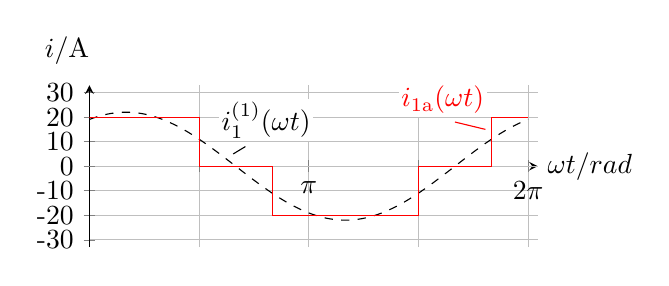
\begin{tikzpicture}
            \begin{axis}[
                % x/y range adjustment
                xmin=0, xmax=368,
                ymin=-33, ymax=33,
                samples=500,
                axis y line=center,
                axis x line=middle,
                extra y ticks=0,
                % Label text
                xlabel={$\omega t / \text{rad}$},,
                ylabel={$i/\mathrm{A}$},
                % Label adjustment
                x label style={at={(axis description cs:1,0.5)},anchor=west},
                y label style={at={(axis description cs:-.05,.97)},anchor=south,yshift=0.2cm},
                width=0.6\textwidth,
                height=0.3\textwidth,
                % x-Ticks
                xtick={0,90,180,270,360},
                xticklabels={,,$\pi$,,$2\pi$},
                xticklabel style = {anchor=north},
                % y-Ticks
                ytick={30,20,10,0,-10,-20,-30},
                yticklabels={30,20,10,0,-10,-20,-30},
                yticklabel style = {anchor=east},
                % Grid layout
                grid,
                %grid style={line width=.1pt, draw=gray!10},
                %major grid style={line width=.2pt,draw=gray!90},
            ]
            % Current i1 fundamentel
            \addplot[black, domain= 0:360,dashed] {22*cos(x-30)};                
            % Current i1d
            \addplot[color=red,solid] coordinates{
                (0, 20)
                (90, 20)
                (90, 0)
                (150, 0)
                (150, -20)
                (270, -20)
                (270, 0)
                (330, 0)
                (330, 20)
                (360, 20)
            };     
        
            % Label of i1a
            \node[red, fill=white, inner sep = 1pt, anchor = south] at (axis cs:290,20) {$i_{\mathrm{1a}}(\omega t)$};
            % Line to i1a
            \draw[thin, red] (325,15) -- (300,18); 
            % Label of i1afundamental
            \node[black, fill=white, inner sep = 1pt, anchor = south] at (axis cs:145,10) {$i_\mathrm{1}^\mathrm{(1)}(\omega t)$};
            % Line to u1a
            \draw[thin, black] (128,8) -- (118,5);             
        \end{axis}     
        \end{tikzpicture}
        \caption{Output current $i_\mathrm{1a}(t)$ and it's fundamental amplitude for raising load.}
        \label{sfig:ex06_Current_i1a_Up}
\end{solutionfigure}